\PosterSection{3. MÉTODOS}
\PosterBody
\begin{posteritems}
  \item \textbf{Dados:} 60 amostras georreferenciadas; treino ampliado para 600 amostras por aumento gaussiano controlado ($\sigma=0{,}01$). As amostras sintéticas não representam novas medições de campo.
  \item \textbf{Entradas:} UTM, temperatura, cor aparente e índice visual de cor.
  \item \textbf{Modelo:} SNN $5 \rightarrow 64 \rightarrow 3$ com LIF, codificação temporal e MSE ponderada.
  \item \textbf{Avaliação:} dez sementes por \textit{repeated random subsampling}; não equivale a validação \textit{k}-fold completa.
\end{posteritems}

\begin{center}
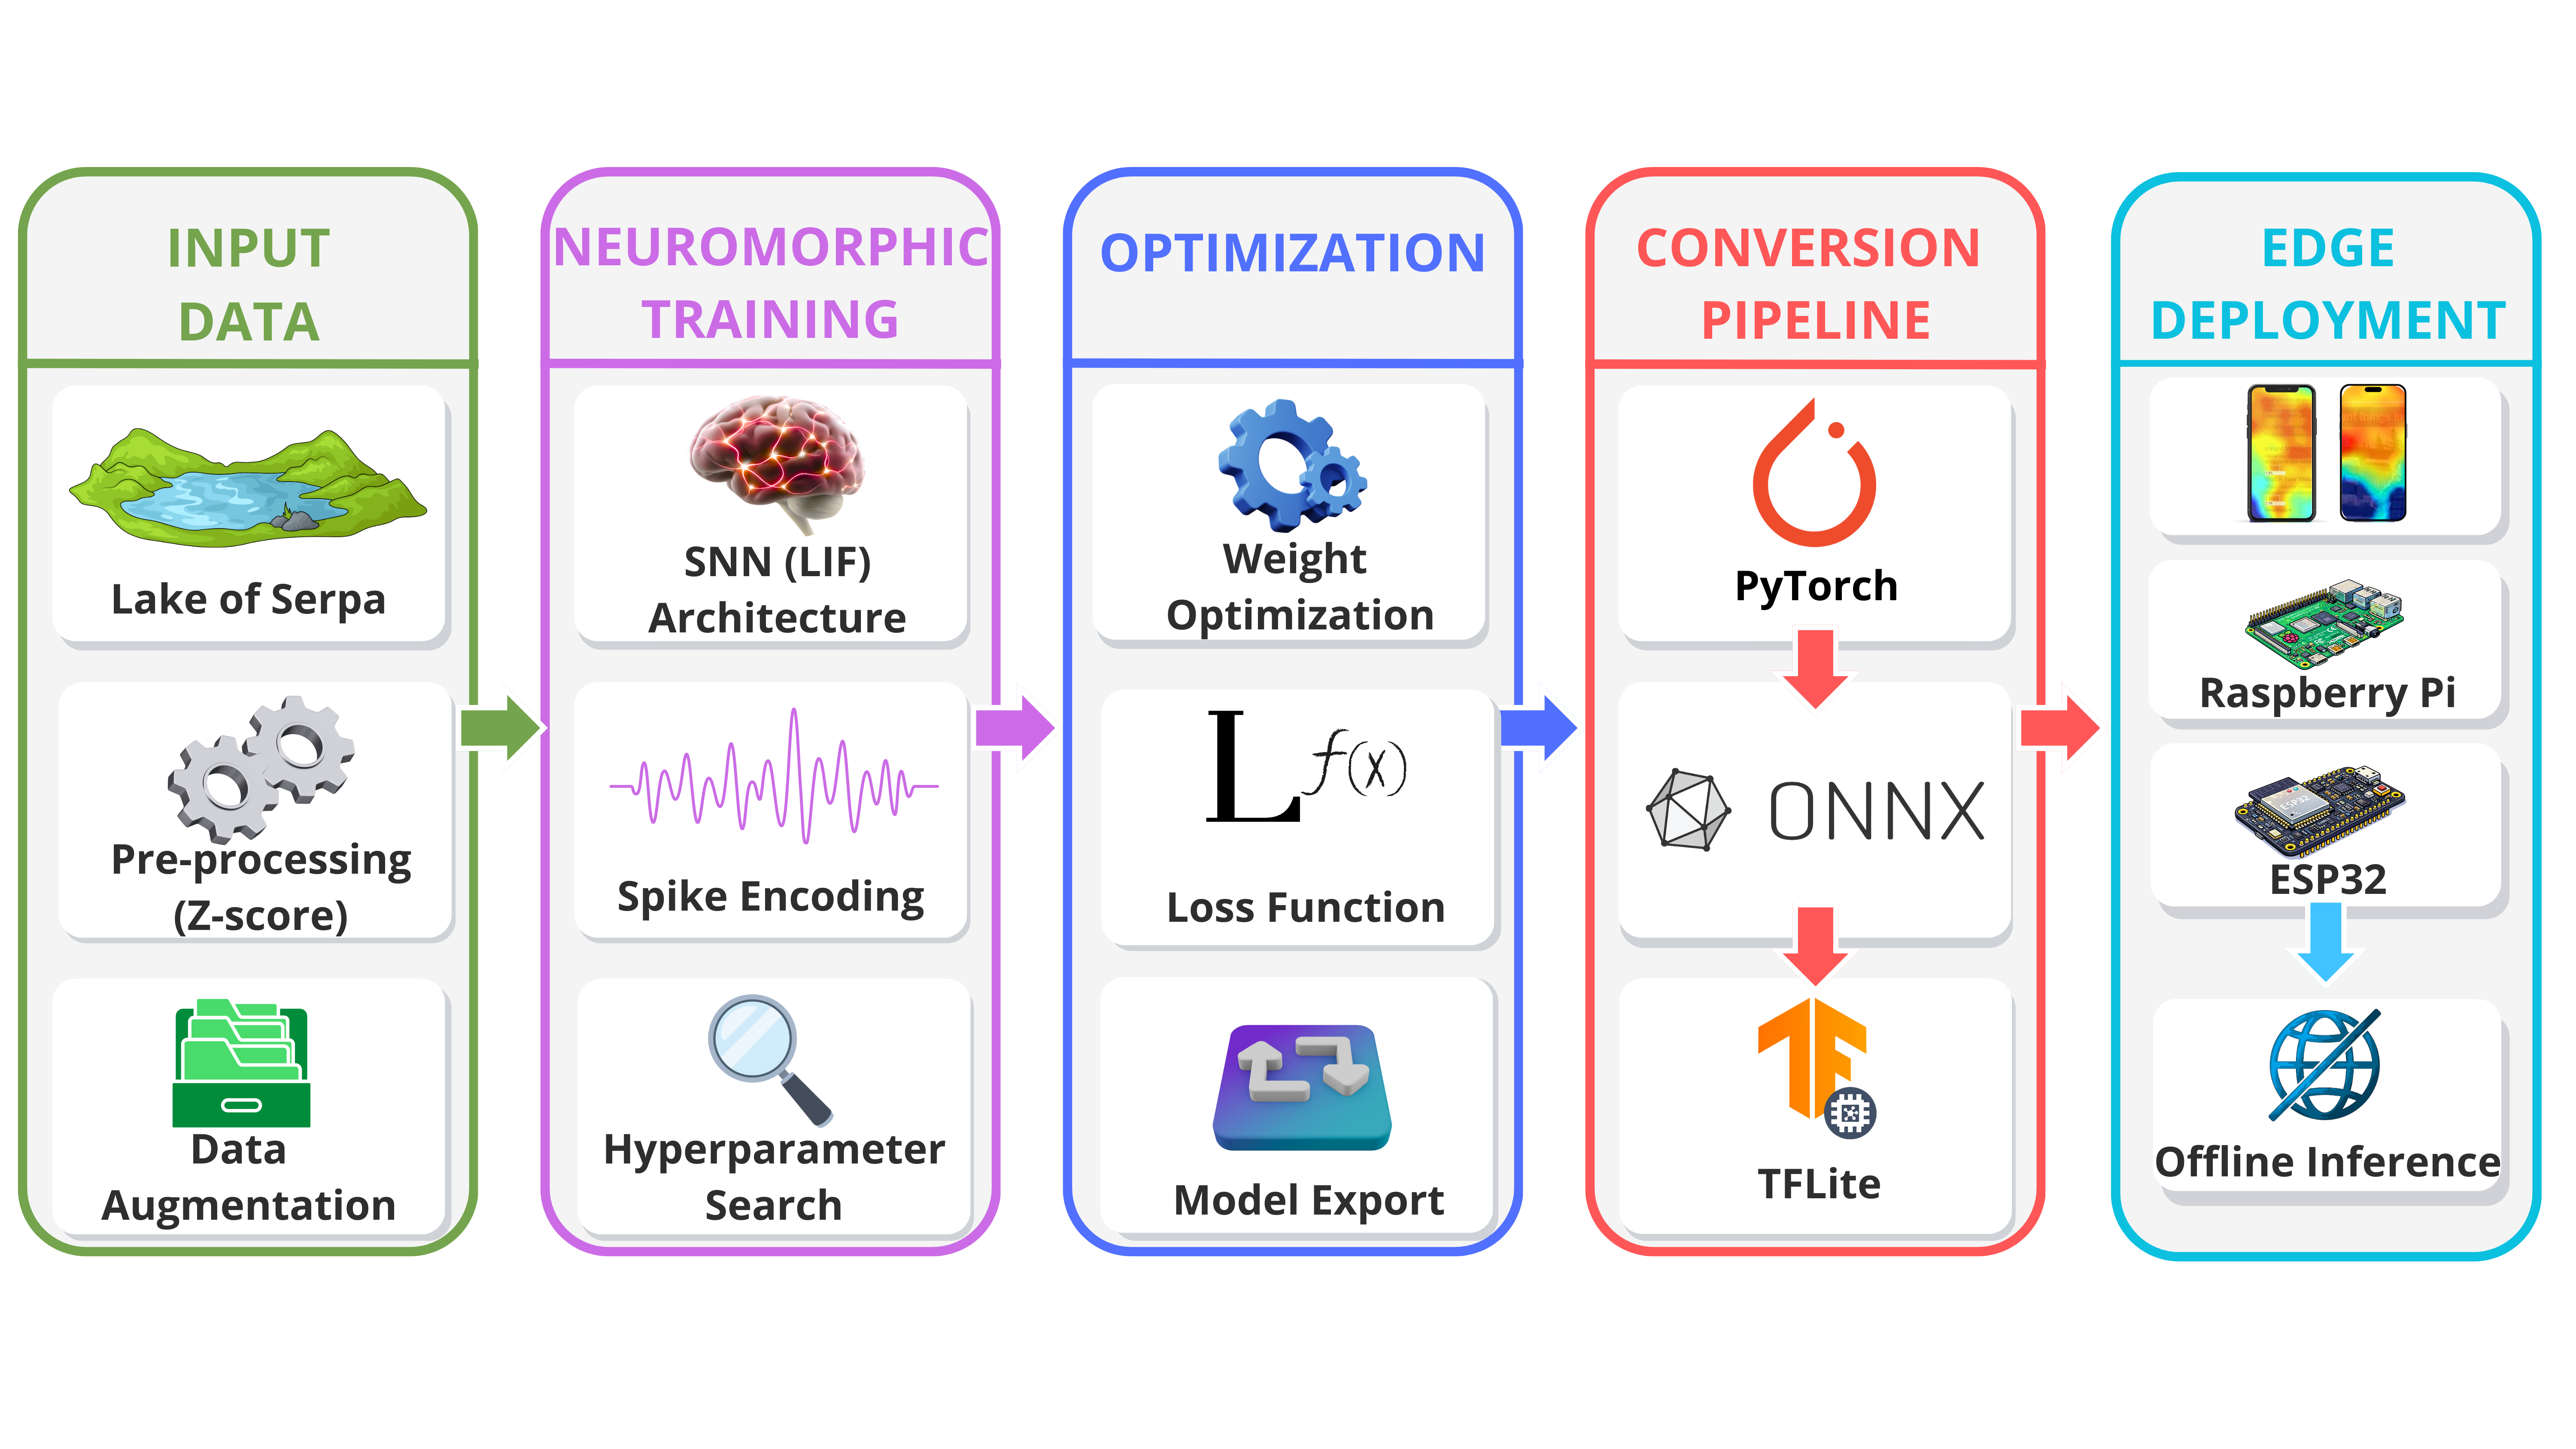
\includegraphics[width=0.70\linewidth]{Arquitetura.png}
\end{center}
\FigureSource{Pipeline SNN multimodal e implantação offline.}
